\documentclass[12pt]{article}
\usepackage{tocloft}
\usepackage{natbib}
\usepackage{url}
\usepackage[utf8x]{inputenc}
\usepackage{amsmath}
\usepackage{graphicx}
\usepackage{verbatim}
\graphicspath{{images/}}
\usepackage{parskip}
\usepackage{fancyhdr}
\usepackage{vmargin}
\setmarginsrb{3 cm}{2.5 cm}{3 cm}{2.5 cm}{1 cm}{1.5 cm}{1 cm}{1.5 cm}
\usepackage{appendix}
\usepackage{listings} % For code importing
\usepackage{xcolor} % for setting colors
 %%%%%%%%%%%%%%%%%%%%%%%%%%%%%%%%%%%%%%%%%%%%%%%%%%%%%%%%%%%%%%%%%%%%%%%%%%%%%%%% 
%%% ~ Arduino Language - Arduino IDE Colors ~                                  %%%
%%%                                                                            %%%
%%% Kyle Rocha-Brownell | 10/2/2017 | No Licence                               %%%
%%% -------------------------------------------------------------------------- %%%
%%%                                                                            %%%
%%% Place this file in your working directory (next to the latex file you're   %%%
%%% working on).  To add it to your project, place:                            %%%
%%%     %%%%%%%%%%%%%%%%%%%%%%%%%%%%%%%%%%%%%%%%%%%%%%%%%%%%%%%%%%%%%%%%%%%%%%%%%%%%%%%% 
%%% ~ Arduino Language - Arduino IDE Colors ~                                  %%%
%%%                                                                            %%%
%%% Kyle Rocha-Brownell | 10/2/2017 | No Licence                               %%%
%%% -------------------------------------------------------------------------- %%%
%%%                                                                            %%%
%%% Place this file in your working directory (next to the latex file you're   %%%
%%% working on).  To add it to your project, place:                            %%%
%%%     %%%%%%%%%%%%%%%%%%%%%%%%%%%%%%%%%%%%%%%%%%%%%%%%%%%%%%%%%%%%%%%%%%%%%%%%%%%%%%%% 
%%% ~ Arduino Language - Arduino IDE Colors ~                                  %%%
%%%                                                                            %%%
%%% Kyle Rocha-Brownell | 10/2/2017 | No Licence                               %%%
%%% -------------------------------------------------------------------------- %%%
%%%                                                                            %%%
%%% Place this file in your working directory (next to the latex file you're   %%%
%%% working on).  To add it to your project, place:                            %%%
%%%    \input{arduinoLanguage.tex}                                             %%%
%%% somewhere before \begin{document} in your latex file.                      %%%
%%%                                                                            %%%
%%% In your document, place your arduino code between:                         %%%
%%%   \begin{lstlisting}[language=Arduino]                                     %%%
%%% and:                                                                       %%%
%%%   \end{lstlisting}                                                         %%%
%%%                                                                            %%%
%%% Or create your own style to add non-built-in functions and variables.      %%%
%%%                                                                            %%%
 %%%%%%%%%%%%%%%%%%%%%%%%%%%%%%%%%%%%%%%%%%%%%%%%%%%%%%%%%%%%%%%%%%%%%%%%%%%%%%%% 

\usepackage{color}
\usepackage{listings}    
\usepackage{courier}

%%% Define Custom IDE Colors %%%
\definecolor{arduinoGreen}    {rgb} {0.17, 0.43, 0.01}
\definecolor{arduinoGrey}     {rgb} {0.47, 0.47, 0.33}
\definecolor{arduinoOrange}   {rgb} {0.8 , 0.4 , 0   }
\definecolor{arduinoBlue}     {rgb} {0.01, 0.61, 0.98}
\definecolor{arduinoDarkBlue} {rgb} {0.0 , 0.2 , 0.5 }

%%% Define Arduino Language %%%
\lstdefinelanguage{Arduino}{
  language=C++, % begin with default C++ settings 
%
%
  %%% Keyword Color Group 1 %%%  (called KEYWORD3 by arduino)
  keywordstyle=\color{arduinoGreen},   
  deletekeywords={  % remove all arduino keywords that might be in c++
                break, case, override, final, continue, default, do, else, for, 
                if, return, goto, switch, throw, try, while, setup, loop, export, 
                not, or, and, xor, include, define, elif, else, error, if, ifdef, 
                ifndef, pragma, warning,
                HIGH, LOW, INPUT, INPUT_PULLUP, OUTPUT, DEC, BIN, HEX, OCT, PI, 
                HALF_PI, TWO_PI, LSBFIRST, MSBFIRST, CHANGE, FALLING, RISING, 
                DEFAULT, EXTERNAL, INTERNAL, INTERNAL1V1, INTERNAL2V56, LED_BUILTIN, 
                LED_BUILTIN_RX, LED_BUILTIN_TX, DIGITAL_MESSAGE, FIRMATA_STRING, 
                ANALOG_MESSAGE, REPORT_DIGITAL, REPORT_ANALOG, SET_PIN_MODE, 
                SYSTEM_RESET, SYSEX_START, auto, int8_t, int16_t, int32_t, int64_t, 
                uint8_t, uint16_t, uint32_t, uint64_t, char16_t, char32_t, operator, 
                enum, delete, bool, boolean, byte, char, const, false, float, double, 
                null, NULL, int, long, new, private, protected, public, short, 
                signed, static, volatile, String, void, true, unsigned, word, array, 
                sizeof, dynamic_cast, typedef, const_cast, struct, static_cast, union, 
                friend, extern, class, reinterpret_cast, register, explicit, inline, 
                _Bool, complex, _Complex, _Imaginary, atomic_bool, atomic_char, 
                atomic_schar, atomic_uchar, atomic_short, atomic_ushort, atomic_int, 
                atomic_uint, atomic_long, atomic_ulong, atomic_llong, atomic_ullong, 
                virtual, PROGMEM,
                Serial, Serial1, Serial2, Serial3, SerialUSB, Keyboard, Mouse,
                abs, acos, asin, atan, atan2, ceil, constrain, cos, degrees, exp, 
                floor, log, map, max, min, radians, random, randomSeed, round, sin, 
                sq, sqrt, tan, pow, bitRead, bitWrite, bitSet, bitClear, bit, 
                highByte, lowByte, analogReference, analogRead, 
                analogReadResolution, analogWrite, analogWriteResolution, 
                attachInterrupt, detachInterrupt, digitalPinToInterrupt, delay, 
                delayMicroseconds, digitalWrite, digitalRead, interrupts, millis, 
                micros, noInterrupts, noTone, pinMode, pulseIn, pulseInLong, shiftIn, 
                shiftOut, tone, yield, Stream, begin, end, peek, read, print, 
                println, available, availableForWrite, flush, setTimeout, find, 
                findUntil, parseInt, parseFloat, readBytes, readBytesUntil, readString, 
                readStringUntil, trim, toUpperCase, toLowerCase, charAt, compareTo, 
                concat, endsWith, startsWith, equals, equalsIgnoreCase, getBytes, 
                indexOf, lastIndexOf, length, replace, setCharAt, substring, 
                toCharArray, toInt, press, release, releaseAll, accept, click, move, 
                isPressed, isAlphaNumeric, isAlpha, isAscii, isWhitespace, isControl, 
                isDigit, isGraph, isLowerCase, isPrintable, isPunct, isSpace, 
                isUpperCase, isHexadecimalDigit, 
                }, 
  morekeywords={   % add arduino structures to group 1
                break, case, override, final, continue, default, do, else, for, 
                if, return, goto, switch, throw, try, while, setup, loop, export, 
                not, or, and, xor, include, define, elif, else, error, if, ifdef, 
                ifndef, pragma, warning,
                }, 
% 
%
  %%% Keyword Color Group 2 %%%  (called LITERAL1 by arduino)
  keywordstyle=[2]\color{arduinoBlue},   
  keywords=[2]{   % add variables and dataTypes as 2nd group  
                HIGH, LOW, INPUT, INPUT_PULLUP, OUTPUT, DEC, BIN, HEX, OCT, PI, 
                HALF_PI, TWO_PI, LSBFIRST, MSBFIRST, CHANGE, FALLING, RISING, 
                DEFAULT, EXTERNAL, INTERNAL, INTERNAL1V1, INTERNAL2V56, LED_BUILTIN, 
                LED_BUILTIN_RX, LED_BUILTIN_TX, DIGITAL_MESSAGE, FIRMATA_STRING, 
                ANALOG_MESSAGE, REPORT_DIGITAL, REPORT_ANALOG, SET_PIN_MODE, 
                SYSTEM_RESET, SYSEX_START, auto, int8_t, int16_t, int32_t, int64_t, 
                uint8_t, uint16_t, uint32_t, uint64_t, char16_t, char32_t, operator, 
                enum, delete, bool, boolean, byte, char, const, false, float, double, 
                null, NULL, int, long, new, private, protected, public, short, 
                signed, static, volatile, String, void, true, unsigned, word, array, 
                sizeof, dynamic_cast, typedef, const_cast, struct, static_cast, union, 
                friend, extern, class, reinterpret_cast, register, explicit, inline, 
                _Bool, complex, _Complex, _Imaginary, atomic_bool, atomic_char, 
                atomic_schar, atomic_uchar, atomic_short, atomic_ushort, atomic_int, 
                atomic_uint, atomic_long, atomic_ulong, atomic_llong, atomic_ullong, 
                virtual, PROGMEM,
                },  
% 
%
  %%% Keyword Color Group 3 %%%  (called KEYWORD1 by arduino)
  keywordstyle=[3]\bfseries\color{arduinoOrange},
  keywords=[3]{  % add built-in functions as a 3rd group
                Serial, Serial1, Serial2, Serial3, SerialUSB, Keyboard, Mouse,
                },      
%
%
  %%% Keyword Color Group 4 %%%  (called KEYWORD2 by arduino)
  keywordstyle=[4]\color{arduinoOrange},
  keywords=[4]{  % add more built-in functions as a 4th group
                abs, acos, asin, atan, atan2, ceil, constrain, cos, degrees, exp, 
                floor, log, map, max, min, radians, random, randomSeed, round, sin, 
                sq, sqrt, tan, pow, bitRead, bitWrite, bitSet, bitClear, bit, 
                highByte, lowByte, analogReference, analogRead, 
                analogReadResolution, analogWrite, analogWriteResolution, 
                attachInterrupt, detachInterrupt, digitalPinToInterrupt, delay, 
                delayMicroseconds, digitalWrite, digitalRead, interrupts, millis, 
                micros, noInterrupts, noTone, pinMode, pulseIn, pulseInLong, shiftIn, 
                shiftOut, tone, yield, Stream, begin, end, peek, read, print, 
                println, available, availableForWrite, flush, setTimeout, find, 
                findUntil, parseInt, parseFloat, readBytes, readBytesUntil, readString, 
                readStringUntil, trim, toUpperCase, toLowerCase, charAt, compareTo, 
                concat, endsWith, startsWith, equals, equalsIgnoreCase, getBytes, 
                indexOf, lastIndexOf, length, replace, setCharAt, substring, 
                toCharArray, toInt, press, release, releaseAll, accept, click, move, 
                isPressed, isAlphaNumeric, isAlpha, isAscii, isWhitespace, isControl, 
                isDigit, isGraph, isLowerCase, isPrintable, isPunct, isSpace, 
                isUpperCase, isHexadecimalDigit, 
                },      
%
%
  %%% Set Other Colors %%%
  stringstyle=\color{arduinoDarkBlue},    
  commentstyle=\color{arduinoGrey},    
%          
%   
  %%%% Line Numbering %%%%
   numbers=left,                    
  numbersep=5pt,                   
  numberstyle=\color{arduinoGrey},    
  %stepnumber=2,                      % show every 2 line numbers
%
%
  %%%% Code Box Style %%%%
  breaklines=true,                    % wordwrapping
  tabsize=2,         
  basicstyle=\ttfamily  
}                                             %%%
%%% somewhere before \begin{document} in your latex file.                      %%%
%%%                                                                            %%%
%%% In your document, place your arduino code between:                         %%%
%%%   \begin{lstlisting}[language=Arduino]                                     %%%
%%% and:                                                                       %%%
%%%   \end{lstlisting}                                                         %%%
%%%                                                                            %%%
%%% Or create your own style to add non-built-in functions and variables.      %%%
%%%                                                                            %%%
 %%%%%%%%%%%%%%%%%%%%%%%%%%%%%%%%%%%%%%%%%%%%%%%%%%%%%%%%%%%%%%%%%%%%%%%%%%%%%%%% 

\usepackage{color}
\usepackage{listings}    
\usepackage{courier}

%%% Define Custom IDE Colors %%%
\definecolor{arduinoGreen}    {rgb} {0.17, 0.43, 0.01}
\definecolor{arduinoGrey}     {rgb} {0.47, 0.47, 0.33}
\definecolor{arduinoOrange}   {rgb} {0.8 , 0.4 , 0   }
\definecolor{arduinoBlue}     {rgb} {0.01, 0.61, 0.98}
\definecolor{arduinoDarkBlue} {rgb} {0.0 , 0.2 , 0.5 }

%%% Define Arduino Language %%%
\lstdefinelanguage{Arduino}{
  language=C++, % begin with default C++ settings 
%
%
  %%% Keyword Color Group 1 %%%  (called KEYWORD3 by arduino)
  keywordstyle=\color{arduinoGreen},   
  deletekeywords={  % remove all arduino keywords that might be in c++
                break, case, override, final, continue, default, do, else, for, 
                if, return, goto, switch, throw, try, while, setup, loop, export, 
                not, or, and, xor, include, define, elif, else, error, if, ifdef, 
                ifndef, pragma, warning,
                HIGH, LOW, INPUT, INPUT_PULLUP, OUTPUT, DEC, BIN, HEX, OCT, PI, 
                HALF_PI, TWO_PI, LSBFIRST, MSBFIRST, CHANGE, FALLING, RISING, 
                DEFAULT, EXTERNAL, INTERNAL, INTERNAL1V1, INTERNAL2V56, LED_BUILTIN, 
                LED_BUILTIN_RX, LED_BUILTIN_TX, DIGITAL_MESSAGE, FIRMATA_STRING, 
                ANALOG_MESSAGE, REPORT_DIGITAL, REPORT_ANALOG, SET_PIN_MODE, 
                SYSTEM_RESET, SYSEX_START, auto, int8_t, int16_t, int32_t, int64_t, 
                uint8_t, uint16_t, uint32_t, uint64_t, char16_t, char32_t, operator, 
                enum, delete, bool, boolean, byte, char, const, false, float, double, 
                null, NULL, int, long, new, private, protected, public, short, 
                signed, static, volatile, String, void, true, unsigned, word, array, 
                sizeof, dynamic_cast, typedef, const_cast, struct, static_cast, union, 
                friend, extern, class, reinterpret_cast, register, explicit, inline, 
                _Bool, complex, _Complex, _Imaginary, atomic_bool, atomic_char, 
                atomic_schar, atomic_uchar, atomic_short, atomic_ushort, atomic_int, 
                atomic_uint, atomic_long, atomic_ulong, atomic_llong, atomic_ullong, 
                virtual, PROGMEM,
                Serial, Serial1, Serial2, Serial3, SerialUSB, Keyboard, Mouse,
                abs, acos, asin, atan, atan2, ceil, constrain, cos, degrees, exp, 
                floor, log, map, max, min, radians, random, randomSeed, round, sin, 
                sq, sqrt, tan, pow, bitRead, bitWrite, bitSet, bitClear, bit, 
                highByte, lowByte, analogReference, analogRead, 
                analogReadResolution, analogWrite, analogWriteResolution, 
                attachInterrupt, detachInterrupt, digitalPinToInterrupt, delay, 
                delayMicroseconds, digitalWrite, digitalRead, interrupts, millis, 
                micros, noInterrupts, noTone, pinMode, pulseIn, pulseInLong, shiftIn, 
                shiftOut, tone, yield, Stream, begin, end, peek, read, print, 
                println, available, availableForWrite, flush, setTimeout, find, 
                findUntil, parseInt, parseFloat, readBytes, readBytesUntil, readString, 
                readStringUntil, trim, toUpperCase, toLowerCase, charAt, compareTo, 
                concat, endsWith, startsWith, equals, equalsIgnoreCase, getBytes, 
                indexOf, lastIndexOf, length, replace, setCharAt, substring, 
                toCharArray, toInt, press, release, releaseAll, accept, click, move, 
                isPressed, isAlphaNumeric, isAlpha, isAscii, isWhitespace, isControl, 
                isDigit, isGraph, isLowerCase, isPrintable, isPunct, isSpace, 
                isUpperCase, isHexadecimalDigit, 
                }, 
  morekeywords={   % add arduino structures to group 1
                break, case, override, final, continue, default, do, else, for, 
                if, return, goto, switch, throw, try, while, setup, loop, export, 
                not, or, and, xor, include, define, elif, else, error, if, ifdef, 
                ifndef, pragma, warning,
                }, 
% 
%
  %%% Keyword Color Group 2 %%%  (called LITERAL1 by arduino)
  keywordstyle=[2]\color{arduinoBlue},   
  keywords=[2]{   % add variables and dataTypes as 2nd group  
                HIGH, LOW, INPUT, INPUT_PULLUP, OUTPUT, DEC, BIN, HEX, OCT, PI, 
                HALF_PI, TWO_PI, LSBFIRST, MSBFIRST, CHANGE, FALLING, RISING, 
                DEFAULT, EXTERNAL, INTERNAL, INTERNAL1V1, INTERNAL2V56, LED_BUILTIN, 
                LED_BUILTIN_RX, LED_BUILTIN_TX, DIGITAL_MESSAGE, FIRMATA_STRING, 
                ANALOG_MESSAGE, REPORT_DIGITAL, REPORT_ANALOG, SET_PIN_MODE, 
                SYSTEM_RESET, SYSEX_START, auto, int8_t, int16_t, int32_t, int64_t, 
                uint8_t, uint16_t, uint32_t, uint64_t, char16_t, char32_t, operator, 
                enum, delete, bool, boolean, byte, char, const, false, float, double, 
                null, NULL, int, long, new, private, protected, public, short, 
                signed, static, volatile, String, void, true, unsigned, word, array, 
                sizeof, dynamic_cast, typedef, const_cast, struct, static_cast, union, 
                friend, extern, class, reinterpret_cast, register, explicit, inline, 
                _Bool, complex, _Complex, _Imaginary, atomic_bool, atomic_char, 
                atomic_schar, atomic_uchar, atomic_short, atomic_ushort, atomic_int, 
                atomic_uint, atomic_long, atomic_ulong, atomic_llong, atomic_ullong, 
                virtual, PROGMEM,
                },  
% 
%
  %%% Keyword Color Group 3 %%%  (called KEYWORD1 by arduino)
  keywordstyle=[3]\bfseries\color{arduinoOrange},
  keywords=[3]{  % add built-in functions as a 3rd group
                Serial, Serial1, Serial2, Serial3, SerialUSB, Keyboard, Mouse,
                },      
%
%
  %%% Keyword Color Group 4 %%%  (called KEYWORD2 by arduino)
  keywordstyle=[4]\color{arduinoOrange},
  keywords=[4]{  % add more built-in functions as a 4th group
                abs, acos, asin, atan, atan2, ceil, constrain, cos, degrees, exp, 
                floor, log, map, max, min, radians, random, randomSeed, round, sin, 
                sq, sqrt, tan, pow, bitRead, bitWrite, bitSet, bitClear, bit, 
                highByte, lowByte, analogReference, analogRead, 
                analogReadResolution, analogWrite, analogWriteResolution, 
                attachInterrupt, detachInterrupt, digitalPinToInterrupt, delay, 
                delayMicroseconds, digitalWrite, digitalRead, interrupts, millis, 
                micros, noInterrupts, noTone, pinMode, pulseIn, pulseInLong, shiftIn, 
                shiftOut, tone, yield, Stream, begin, end, peek, read, print, 
                println, available, availableForWrite, flush, setTimeout, find, 
                findUntil, parseInt, parseFloat, readBytes, readBytesUntil, readString, 
                readStringUntil, trim, toUpperCase, toLowerCase, charAt, compareTo, 
                concat, endsWith, startsWith, equals, equalsIgnoreCase, getBytes, 
                indexOf, lastIndexOf, length, replace, setCharAt, substring, 
                toCharArray, toInt, press, release, releaseAll, accept, click, move, 
                isPressed, isAlphaNumeric, isAlpha, isAscii, isWhitespace, isControl, 
                isDigit, isGraph, isLowerCase, isPrintable, isPunct, isSpace, 
                isUpperCase, isHexadecimalDigit, 
                },      
%
%
  %%% Set Other Colors %%%
  stringstyle=\color{arduinoDarkBlue},    
  commentstyle=\color{arduinoGrey},    
%          
%   
  %%%% Line Numbering %%%%
   numbers=left,                    
  numbersep=5pt,                   
  numberstyle=\color{arduinoGrey},    
  %stepnumber=2,                      % show every 2 line numbers
%
%
  %%%% Code Box Style %%%%
  breaklines=true,                    % wordwrapping
  tabsize=2,         
  basicstyle=\ttfamily  
}                                             %%%
%%% somewhere before \begin{document} in your latex file.                      %%%
%%%                                                                            %%%
%%% In your document, place your arduino code between:                         %%%
%%%   \begin{lstlisting}[language=Arduino]                                     %%%
%%% and:                                                                       %%%
%%%   \end{lstlisting}                                                         %%%
%%%                                                                            %%%
%%% Or create your own style to add non-built-in functions and variables.      %%%
%%%                                                                            %%%
 %%%%%%%%%%%%%%%%%%%%%%%%%%%%%%%%%%%%%%%%%%%%%%%%%%%%%%%%%%%%%%%%%%%%%%%%%%%%%%%% 

\usepackage{color}
\usepackage{listings}    
\usepackage{courier}

%%% Define Custom IDE Colors %%%
\definecolor{arduinoGreen}    {rgb} {0.17, 0.43, 0.01}
\definecolor{arduinoGrey}     {rgb} {0.47, 0.47, 0.33}
\definecolor{arduinoOrange}   {rgb} {0.8 , 0.4 , 0   }
\definecolor{arduinoBlue}     {rgb} {0.01, 0.61, 0.98}
\definecolor{arduinoDarkBlue} {rgb} {0.0 , 0.2 , 0.5 }

%%% Define Arduino Language %%%
\lstdefinelanguage{Arduino}{
  language=C++, % begin with default C++ settings 
%
%
  %%% Keyword Color Group 1 %%%  (called KEYWORD3 by arduino)
  keywordstyle=\color{arduinoGreen},   
  deletekeywords={  % remove all arduino keywords that might be in c++
                break, case, override, final, continue, default, do, else, for, 
                if, return, goto, switch, throw, try, while, setup, loop, export, 
                not, or, and, xor, include, define, elif, else, error, if, ifdef, 
                ifndef, pragma, warning,
                HIGH, LOW, INPUT, INPUT_PULLUP, OUTPUT, DEC, BIN, HEX, OCT, PI, 
                HALF_PI, TWO_PI, LSBFIRST, MSBFIRST, CHANGE, FALLING, RISING, 
                DEFAULT, EXTERNAL, INTERNAL, INTERNAL1V1, INTERNAL2V56, LED_BUILTIN, 
                LED_BUILTIN_RX, LED_BUILTIN_TX, DIGITAL_MESSAGE, FIRMATA_STRING, 
                ANALOG_MESSAGE, REPORT_DIGITAL, REPORT_ANALOG, SET_PIN_MODE, 
                SYSTEM_RESET, SYSEX_START, auto, int8_t, int16_t, int32_t, int64_t, 
                uint8_t, uint16_t, uint32_t, uint64_t, char16_t, char32_t, operator, 
                enum, delete, bool, boolean, byte, char, const, false, float, double, 
                null, NULL, int, long, new, private, protected, public, short, 
                signed, static, volatile, String, void, true, unsigned, word, array, 
                sizeof, dynamic_cast, typedef, const_cast, struct, static_cast, union, 
                friend, extern, class, reinterpret_cast, register, explicit, inline, 
                _Bool, complex, _Complex, _Imaginary, atomic_bool, atomic_char, 
                atomic_schar, atomic_uchar, atomic_short, atomic_ushort, atomic_int, 
                atomic_uint, atomic_long, atomic_ulong, atomic_llong, atomic_ullong, 
                virtual, PROGMEM,
                Serial, Serial1, Serial2, Serial3, SerialUSB, Keyboard, Mouse,
                abs, acos, asin, atan, atan2, ceil, constrain, cos, degrees, exp, 
                floor, log, map, max, min, radians, random, randomSeed, round, sin, 
                sq, sqrt, tan, pow, bitRead, bitWrite, bitSet, bitClear, bit, 
                highByte, lowByte, analogReference, analogRead, 
                analogReadResolution, analogWrite, analogWriteResolution, 
                attachInterrupt, detachInterrupt, digitalPinToInterrupt, delay, 
                delayMicroseconds, digitalWrite, digitalRead, interrupts, millis, 
                micros, noInterrupts, noTone, pinMode, pulseIn, pulseInLong, shiftIn, 
                shiftOut, tone, yield, Stream, begin, end, peek, read, print, 
                println, available, availableForWrite, flush, setTimeout, find, 
                findUntil, parseInt, parseFloat, readBytes, readBytesUntil, readString, 
                readStringUntil, trim, toUpperCase, toLowerCase, charAt, compareTo, 
                concat, endsWith, startsWith, equals, equalsIgnoreCase, getBytes, 
                indexOf, lastIndexOf, length, replace, setCharAt, substring, 
                toCharArray, toInt, press, release, releaseAll, accept, click, move, 
                isPressed, isAlphaNumeric, isAlpha, isAscii, isWhitespace, isControl, 
                isDigit, isGraph, isLowerCase, isPrintable, isPunct, isSpace, 
                isUpperCase, isHexadecimalDigit, 
                }, 
  morekeywords={   % add arduino structures to group 1
                break, case, override, final, continue, default, do, else, for, 
                if, return, goto, switch, throw, try, while, setup, loop, export, 
                not, or, and, xor, include, define, elif, else, error, if, ifdef, 
                ifndef, pragma, warning,
                }, 
% 
%
  %%% Keyword Color Group 2 %%%  (called LITERAL1 by arduino)
  keywordstyle=[2]\color{arduinoBlue},   
  keywords=[2]{   % add variables and dataTypes as 2nd group  
                HIGH, LOW, INPUT, INPUT_PULLUP, OUTPUT, DEC, BIN, HEX, OCT, PI, 
                HALF_PI, TWO_PI, LSBFIRST, MSBFIRST, CHANGE, FALLING, RISING, 
                DEFAULT, EXTERNAL, INTERNAL, INTERNAL1V1, INTERNAL2V56, LED_BUILTIN, 
                LED_BUILTIN_RX, LED_BUILTIN_TX, DIGITAL_MESSAGE, FIRMATA_STRING, 
                ANALOG_MESSAGE, REPORT_DIGITAL, REPORT_ANALOG, SET_PIN_MODE, 
                SYSTEM_RESET, SYSEX_START, auto, int8_t, int16_t, int32_t, int64_t, 
                uint8_t, uint16_t, uint32_t, uint64_t, char16_t, char32_t, operator, 
                enum, delete, bool, boolean, byte, char, const, false, float, double, 
                null, NULL, int, long, new, private, protected, public, short, 
                signed, static, volatile, String, void, true, unsigned, word, array, 
                sizeof, dynamic_cast, typedef, const_cast, struct, static_cast, union, 
                friend, extern, class, reinterpret_cast, register, explicit, inline, 
                _Bool, complex, _Complex, _Imaginary, atomic_bool, atomic_char, 
                atomic_schar, atomic_uchar, atomic_short, atomic_ushort, atomic_int, 
                atomic_uint, atomic_long, atomic_ulong, atomic_llong, atomic_ullong, 
                virtual, PROGMEM,
                },  
% 
%
  %%% Keyword Color Group 3 %%%  (called KEYWORD1 by arduino)
  keywordstyle=[3]\bfseries\color{arduinoOrange},
  keywords=[3]{  % add built-in functions as a 3rd group
                Serial, Serial1, Serial2, Serial3, SerialUSB, Keyboard, Mouse,
                },      
%
%
  %%% Keyword Color Group 4 %%%  (called KEYWORD2 by arduino)
  keywordstyle=[4]\color{arduinoOrange},
  keywords=[4]{  % add more built-in functions as a 4th group
                abs, acos, asin, atan, atan2, ceil, constrain, cos, degrees, exp, 
                floor, log, map, max, min, radians, random, randomSeed, round, sin, 
                sq, sqrt, tan, pow, bitRead, bitWrite, bitSet, bitClear, bit, 
                highByte, lowByte, analogReference, analogRead, 
                analogReadResolution, analogWrite, analogWriteResolution, 
                attachInterrupt, detachInterrupt, digitalPinToInterrupt, delay, 
                delayMicroseconds, digitalWrite, digitalRead, interrupts, millis, 
                micros, noInterrupts, noTone, pinMode, pulseIn, pulseInLong, shiftIn, 
                shiftOut, tone, yield, Stream, begin, end, peek, read, print, 
                println, available, availableForWrite, flush, setTimeout, find, 
                findUntil, parseInt, parseFloat, readBytes, readBytesUntil, readString, 
                readStringUntil, trim, toUpperCase, toLowerCase, charAt, compareTo, 
                concat, endsWith, startsWith, equals, equalsIgnoreCase, getBytes, 
                indexOf, lastIndexOf, length, replace, setCharAt, substring, 
                toCharArray, toInt, press, release, releaseAll, accept, click, move, 
                isPressed, isAlphaNumeric, isAlpha, isAscii, isWhitespace, isControl, 
                isDigit, isGraph, isLowerCase, isPrintable, isPunct, isSpace, 
                isUpperCase, isHexadecimalDigit, 
                },      
%
%
  %%% Set Other Colors %%%
  stringstyle=\color{arduinoDarkBlue},    
  commentstyle=\color{arduinoGrey},    
%          
%   
  %%%% Line Numbering %%%%
   numbers=left,                    
  numbersep=5pt,                   
  numberstyle=\color{arduinoGrey},    
  %stepnumber=2,                      % show every 2 line numbers
%
%
  %%%% Code Box Style %%%%
  breaklines=true,                    % wordwrapping
  tabsize=2,         
  basicstyle=\ttfamily  
}  


\begin{document}
\title{Project Report}
%%%%%%%%%%%%%%%%%%%%%%%%%%%%%%%%%%%%%%%%%%%%%%%%%%%%%%%%%%%%%%%%%%%%%%%%%%%%%%%%%%%%%%%%%

\begin{titlepage}
\centering
    \vspace*{0.5 cm}
    
\includegraphics[scale = 0.11]{isu_seal.png}\\[1.0 cm] % University Logo
    \textsc{\LARGE IOWA STATE UNIVERSITY}\\[2.0 cm]
    \textsc{\large AEROSPACE ENGINEERING DEPARTMENT}\\[0.2 cm]
    \textsc{\large Computational Techniques for Aerospace Design}\\[0.2 cm]
\textsc{\Large AERE 361}\\[0.5 cm] % Course Code
\textsc{\Large Spring 2021}\\[0.5 cm] % Course Code
\textsc{\Large Final Project Report}\\[0.2 cm]
\textsc{\Large The Fourteeners}\\[0.2 cm]
\rule{\linewidth}{0.2 mm} \\[0.4 cm]
%{ \huge \bfseries \thetitle}\\


\begin{minipage}{0.8\textwidth}

\begin{flushleft}
\emph{Team Member Names :} \\
Cashen, William\linebreak
Hood, Delane\linebreak
Winter, Alex\linebreak
Kapoor, Khushi\linebreak
\end{flushleft}
\end{minipage}\\[2 cm]

\vfill

\end{titlepage}

%%%%%%%%%%%%%%%%%%%%%%%%%%%%%%%%%%%%%%%%%%%%%%%%%%%%%%%%%%%%%%%%%%%%%%%%%%%%%%%%%%%%%%%%%
%\maketitle
\tableofcontents
\pagebreak
%%%%%%%%%%%%%%%%%%%%%%%%%%%%%%%%%%%%%%%%%%%%%%%%%%%%%%%%%%%%%%%%%%%%%%%%%%%%%%%%%%%%%%%%%

\section{ABSTRACT}
%Will-Also put and format images into project.
This year the students of AerE 361 were tasked with solving a problem using a circuit playground express(CPX) board.
For many of us, this was the first time working and testing hardware while simultaneously working on its code. We originally
were meant to be exposed to this during freshman year with the butter tray robots, but unfortunately COVID put a lid on that.
Our group `The Fourteeners' wanted to have some fun with the project so we took a real life concern for a modern day soccer player
and shrunk it down to LEGO size. Below we will walk through what exactly we solved using the CPX and how we went about doing so.
There will also be a reflection section where we talk about the status, lessons learned, our results, and things moving forward.
\section{INTRODUCTION}
The Fourteeners group decided to create a penalty kick simulator for Lionel Messi. Based on research, over Messi's career, he has missed a higher percentage of penalty kicks that Christiano Ronaldo. Because of this, we decided to design and execute a simulator that will allow Messi to practice his shots. The research that was done found that certain areas of the goal are more likely to be scored in, so sensors were placed in those spots to provide Messi with positive feedback.

The members of this group are Will Cashen, Alex Winter, Delane Hood and Khushi Kapoor. All four of the members worked very closely to see this project from start to finish. As the team lead, Will oversaw the progress of the team and also did a lot of work on the programming. Khushi assisted Will with the project oversight as well as focused on the features that would be integrated in the physical model. Alex focused on the combination of all the codes of the features together. Delane used his strong arduino knowledge to assist with the project as a whole as well as helped Khushi with the physical model. 
\section{FEATURES}
There were 5 main features that were used for our project. This list of features changed drastically throughout the semester. The few other components we were originally hoping to have in the project were a 7-segment display, possibly using LEDs, and even the possibility of using another servo to control lateral movement of the kicker. 

The first step in our project is using a joystick to control Messi's kick. Instead of using it is a joystick however, we used the push sensor capability to automate the kick. The code for this was quite simple and was connected to the movement of the servo. 

Next, the servo was also a main feature of our project. As mentioned above, it controlled the kick by the push on the joystick. We originally did some research into which type of servo we would be needing to use. Even after our research, and trying to see what different setting in our code we could use, we were still running into some issues with the power of the kick so we ended up using some fishing wire to create some torque. 

The third component was the ultrasonic sensor. This sensor was placed at the goal line to detect whether or not the ball went inside the goal. This was a part of our original plan and we are glad it ended up working. We originally had to do some adjustments to make the sensor sensitive enough to pickup the ball moving in front of it. 

The pressure sensors were also an original part of our idea. We placed a pressure sensor in each corner of the goal. This is where a soccer player is most likely to score a goal, according to our research. We did a lot of research and adjustments to try and make these two sensors more sensitive as well, and found that changing the resistance really worked. 

Lastly, the neopixels on the CPX board served as our LEDs/7 segment display idea. Since we were not able to incorporate them due to a shortage of pin connections, we resorted to using the neopixels. As described in the solution, we used different use cases to light up the board with different colors. 


\section{PROBLEM STATEMENT}
We took the real life soccer player Lionel Messi and looked at his penalty kick percentage. According to the statistics reported by Michel Acosta\cite{michelacosta} we saw that he had missed 22 percent of his shots. Not necessarily amazing for the superstar, and not to mention there's always been a question about who's the best player; Ronaldo or Messi? Currently Ronaldo has the better shooting percentage for penalty kicks sitting at 83 percent. In order to change that our group needed to provide Messi with a way to not only practice his penalty kicks, but efficiently choose where to place them in order to score.Using more stats provided by `thestatszone'\cite{StatsZone.com} we figure out where to make the targets to provide a better estimate too our solution. Additionally, lets say we want to make this universal, for other players. We needed to create a feedback system to the let the kicker know the liklieness of scoring on a goalie. This is where the targets and stats come into play.

\section{PROBLEM SOLUTION}%%%%%%%%%%% DELANE START HERE %%%%%%%%%%%%%%%%%%%%%%%%%%%%%%%%%%%%%%%%%%%%%%%%%%%%%%%%%%%%%%%%%%%%%%%%%%%%%%%%%%%%%%%%%%%%%%%%%%%%%%%%%%%%%%%%%%%%%%
% Here, you go into detail what your solution to the problem is.  I expect that this will have several subsections and you should breakout each area.  You should include any graphics and pictures as relevant as well and reference them like Figure \ref{fig:cpx}.

%\begin{itemize}
%    \item How did you come up with your solution
%    \item How did you test or verify your solution
%    \item Do you think this was a good solution?
%    \item Show as much as you can of the solution in action (pictures and/or data)
%\end{itemize}

Our solution was to create a penalty kick simulator for Messi to practice kicks. Messi would use our device to shoot a ball into the goal and it gives feedback on the likeliness that the ball would score based on real FIFA stats. The more that Messi practiced kicks, he would learn good places to aim for his penatly kicks. Our project was split into two areas of control, each with their own Circuit Playground Express(CPX) board. One CPX board controlled the servo to actuate the kick and the joystick to command the kick. The other CPX relayed information from two pressure sensors and an ultrasonic sensor to the on-board LEDs to display the kick accuracy. We Used two CPX boards because one didn't have enough pin outs to control all of the hardware we were using. Below in each section gives further detail on how each CPX is set up. 

\subsection{Kicking control CPX}

A two axis joystick was used to start the kicking action with a downward button press. The original idea was to have the joystick move the kicker left and right, similar to a Foosball Table. The other axis on the joystick was going to be used to adjust the kicking power. However, due to time and hardware constraints we were not able to implement them in the final design. The joystick ended up only needed one pin out for the button press. Below in Figure \ref{fig:left} you can see the joystick near the bottom of the image plugged in to the bread board. 

This CPX also controlled a position servo to give the figure his kicking action. We had also planned to use a second servo to have the kicker slide side to side to try different kick positions, but was not implemented for the same reasons stated above. The servo that was connected to the kicker was given mechanical advantage by using a small string to rotate the kicker faster than the rotation of the servo.The servo would be actuated by a press of the joystick described above. One limitation we found of our final design is that the servo was not as quick as we wanted. Below in Figure \ref{fig:left} you can see the servo attached to the rotating kick dowel with an enhanced outline of the string (white lines).

\begin{figure}[!t]
\centering
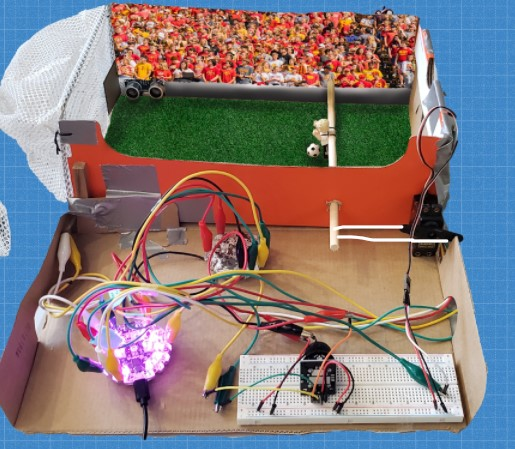
\includegraphics[width=4.5in]{project_left.jpg}
\caption{Left side of project}
\label{fig:left}
\end{figure}


%\begin{figure}[!t]
%\centering
%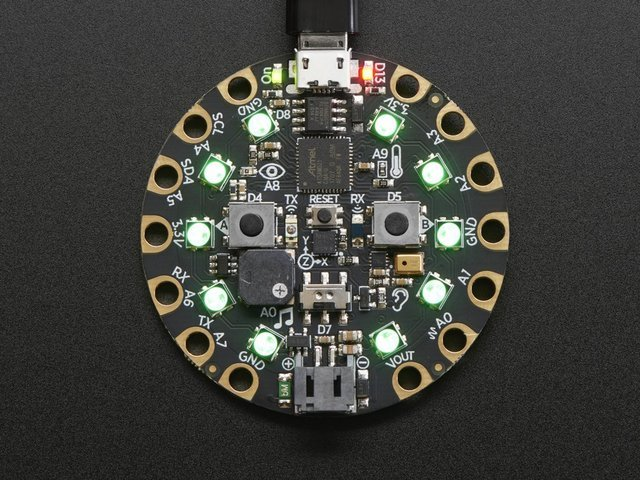
\includegraphics[width=4.5in]{cpx01.jpg}
%\caption{This is the circuit playground express}
%\label{fig:cpx}
%\end{figure}

\subsection{Kick scoring CPX}

This CPX controlled the ultrasonic sensor, two pressure sensors, and the LED feedback systems. The ultrasonic sensor detected movement across the goal line and was able to recognize that a ball had crossed in its path. The pressure sensors were placed in the lower left and right corners of the goal. The pressure sensors were also sensitive enough to detect a quick moving kick and a slow moving kick ball. 

\subsubsection{Sensors used}

The ultrasonic sensor was able to detect the ball crossing into the goal by sending out a high frequency sound and listening for the reflection of the sound and timing the difference between the sent and received signal. We calibrated the sensor with the known distance across the goal. then we used an If statement in our code that if the received signal was shorter than the goal, then it considered the ball as a goal. We were able to get it working by referencing the website tutorials point \cite{tutorialspoint}. %put bib ref here 

The pressure sensors were able to detect a hit by bending from the ball pressing on the free end of the sensor. The sensors we used were Force Sensitive Resistor (FSR). We were able to record the amount of pressure detected and used a cutoff point between when the FSR detected a quick kick and a slow kick. The quicker kick of course created higher pressure. We found a helpful resource on Adafruit's website on how to code and wire the hardware for the FSR \cite{Adafruit}. %put bib ref here 


\subsubsection{Score Conditions}
If the ball passed into the goal without hitting the pressure sensors on the sides, the LEDs would light up purple allowing Messi to know that his kick was placed in the center of the goal and likely to score. Above in Figure \ref{fig:left} you can see the LEDs are purple. If the ball hit one of the pressure sensors in the corner at a slow speed, the LEDs would turn yellow indicating that shot would be less than likely a goal. If the ball hit one of the pressure sensors at a high speed, the LEDs would illuminate green which would indicate a high chance of scoring the shot. 



\subsection{Testing and Verification}

\subsubsection{Ultrasonic}

The ultrasonic sensor was tested with two different types of soccer balls. A small appropriately size Lego ball that matched the size as for the mini-figure and a much larger table tennis ball. Fortunately the sensor was able to pick up the reading from the smaller sized Lego ball. We hypothesized that the ball would be too small to be recognized by the ultrasonic sensor, however the sensor could accurately measure the small soccer ball's position. Another issue we hypothesized about the ultrasonic sensor was that it wouldn't be able to recognize the ball if it were moving too quickly. Yet again the sensor surprised us by recognizing the ball when it was rolled quite quickly into the goal. The ultrasonic sensor surpassed our expectations and worked quite well on testing.  

\subsubsection{FSR}

One early testing issue we had with the FSR was that it wasn't sensitive enough to take a reading of any ball kicked into it. It took a significant amount of force to get the smallest reading from it. We were able to work around the issue by adding more Resistance to the circuit by adding a resistor. Doing this allowed the FSR to take MUCH more sensitive readings thus, allowing us to not only read that the ball hit it, but to be able to differentiate the speed that the soccer ball hit it with. 

\subsubsection{Solution effectiveness}

We agreed that our solution to help Messi with his kicks would be effective on completion. We know that each of the systems on the CPX boards worked well, but only while independently. If we had a bit more time to work out the small issues, we would be sure that it would be an effective solution. The effectiveness of the solution we have so far is ineffective. The status of this project is further detailed in the next section. 

%Again, cite any sources that you have.  If you took snippets of code or found a paper that discusses on how to do something, then you need to cite it. The same if you got inspiration for code from a source, cite that as well. For this final project report, I am expecting at least 3 sources cited.  One will probably be what you had in your problem statement from your proposal.  

%Your problem solution is one of the largest things we look at. I am looking for the following items:

%\begin{itemize}
%    \item How did you come up with your solution
%    \item How did you test or verify your solution
%    \item Do you think this was a good solution?
%    \item Show as much as you can of the solution in action (pictures and/or data)
%\end{itemize}

%For this reason, this section has the most points at 25 points



%%%%%%%%%%%%%%%%%%%%%%%%%%%%%%%%%%%%%%%%%%%%%%%%%%%%%%%%%%%%%%%END-DELANE %%%%%%%%%%%%%%%%%%%%%%%%%%%%%%%%%%%%%%%%%%%%%%%%%%%%%%%%%%%%%%%%%%%%%%%%%%%%%%%%%%%%%%%%%%%%%%%%%%





\section{STATUS}
Throughout the course the project we continually adapted our goals and further refined how the original goals
could be accomplished. This process led to a mostly successful project with a few shortcomings in the 
electronics used. We were a bit too ambitious with using an external LED display and had to drop it from being used in our final presentation due to the number of inputs it required to operate and the simplicity of the Playground Express boards. The servo system we had devised to "kick" the soccer ball was functioning as expected and accomplished its goal within the project and then suddenly stopped working the night before the presentation, the source of the malfunction is unknown, but is assumed to be hardware failure. The ultrasonic sensor seemed to be going through some similar problems with working sometimes and not others without changing usage conditions. The pressure sensors and scoring 'algorithm' we devised functioned properly and accomplished its goal. The implementation with the pressure sensors could have been implemented better using a moving base for conditional statements to determine outcomes based on initial readings. The visible confirmation of a score using the Neopixel lights functioned correctly.

\subsection{Lessons Learned}
A semester-long project like this comes with a lot of lessons learned. To begin, we found that it was very important to ensure clear communication with each other. We decided on a means of communication, and set forth with clear ways to reach each other and decided on a meeting cadence. Additionally, we were able to decide on a team-lead, and whenever Will, our lead, was unable to attend someone else was able to setup. We did not run into any issues with who should be leading the team or the direction we should go in which was great. The programming aspect of this project was a lesson in and of itself. It was a lot of research combined with trial and error to get all of our components to communicate. What we learned from that is to be patient and inquisitive to try and troubleshoot our code. Overall, we learned a lot and worked greatly as a team.

\section{RESULTS}
The data collected for this project was minimal as the project relied on visual representation of whether a score occurred or not. This visual representation can be seen in Figure left in the Solution section where the Playground Express Neopixels are illuminated purple color to demonstrate a goal that missed the pressure sensors. The board was successful in visually demonstrating all four states of an attempted shot on the goal. Red for a total miss, purple for a goal not contacting the pressure sensors, yellow for a soft kicked goal and green for a hard kicked goal. 
The code can be found at the bottom of this report or on the GitHub repository referenced at the bottom of this report. 

\section{FUTURE WORK}
As a team, we briefly discussed possible future work with Professor Nelson. As we described in our presentation, the 3 main things we would hope to work on are the mechanical structure of the soccer field, the servo motor used to kick, and the pressure sensors. For the structure of the field, we found that at times it was hard to recreate each kick due to the cardboard or maybe an imbalance in the field. This could be mitigated if we used a more sturdy field which was built from stronger materials and also made it a little bigger. Secondly, for the servo, we discussed possibly using a motor instead of a servo since that servo isn't really meant for a repetitive rotational motion and would have been better for maybe a translation motion. Lastly, we would work to see if we can do a calibration reset on the pressure sensors that averages the values it gets before every test so that it is calibrated and runs properly. 

\section{CONCLUSION}
For this final project, team The Fourteeners created a soccer simulation with the objective to practice kicking a penalty kick and demonstrate a score or miss to determine the effectiveness of shots into a goal. This project had many successfully functioning components and the system was able to function with "kicking", monitoring the goal line and visually demonstrating whether or not a goal had been scored. The project gave the team great practical knowledge of how the Arduino system can be utilized and how to connect electronic subsystems to create a large functional system. Some improvements could have been made to increase the reliability of the pressure sensor thresholds used to register a score and to increase functionality of the ultrasonic sensor to determine whether a ball cross the goal line threshold. Overall the project was a success and the team worked well together to define a problem and work towards solving it by creating a functional electronic system.

\newpage

\bibliographystyle{plain}
\bibliography{ref}
\newpage
% you need to have at least your code in your appendix
\appendix

\section{SOURCE CODE}
Repo - \url{https://github.com/WilliamTell78/The-Fourteeners-Final-Project.git}
CPX1 - Source Code
\lstinputlisting[language=Arduino]{PressureSensor_UltrasonicSensor_Together.ino}
CPX2 - Source Code
\lstinputlisting[language=Arduino]{Joystick_Merged_with_Servo/Joystick_Merged_with_Servo.ino}

\end{document}
